\chapter{Implementation}
\label{chapter:implementation}

The main part of implementing the parser was to rewrite the EBNF provided by W3C in \cite{w3c01} to conform to ANTLR's syntax and semantics. Because of the ambiguous terminals described in section \ref{sect:ambiguousgrammar:ambigTerm} this was not a trivial task, and in the following chapter we will present by which means we solved this. In addition we will present other how we reduced the parser required lookahead, implemented a parser that mangages a language without reserved keywords, how we augmented the grammar to output a correct AST and finally our implementation of scoping and symbol tables.


\section{ANTLR Syntax Conformity}
The W3C(\cite{w3c00}) and ANTLR(section \ref{sect:antlr:grammarSpec}) EBNF syntax differs in multiple ways. Some of the differences are trivial, e.g. the "defined by"-operator, which in W3C syntax is denoted with \verb!::=! and in ANTLR syntax as \verb!:!. Such differences can be fixed by means of a simple symbol replacement. However, the W3C metagrammar also embodies some operators such as the 'hat' and the 'dash' operators, described in section \ref{sect:ambiguousgrammar:ambigTerm}, of which there are no complete equivalents in the ANTLR metagrammar. In addition, the W3C grammar defines some producions as terminal and other as non-terminal, but this division does not hold for all implementations.

\subsection{Seperating Parser and Lexer Rules}

The ANTLR parser generator can generate parsers and lexers from a single grammar file. The distinction between terminals and non-terminals is that terminals start with \emph{uppercase} letters, and non-terminals start with \emph{lowercase} letters. Which productions to go where is highly dependant on what strategy we chose to solve the ambigious terminals problem. E.g. by defining all the ambigious terminals as non-terminals we would have solution very close to a scan-while-parse scanner (section \ref{sect:ambiguousgrammar:scanWhileParse}). Because we chose the strategy of letting the parser control the lexer's state, we vere able define a division of terminals and non-terminals very similar to the one specified by W3C. The exception is \verb!QName!, which by W3C is defined as follows:
\begin{verbatim}
QName           ::= PrefixedName
                  | UnprefixedName
PrefixedName    ::= Prefix ':' LocalPart 
UnprefixedName  ::= LocalPart 
Prefix          ::= NCName
LocalPart       ::= NCName
\end{verbatim}
Where \verb!NCName! is another terminal, thus creating an ambiguity in the case where \verb!QName! uses the \verb!UnprefixedName! alternative. It is possible to rank the \verb!QName! production higher than the \verb!NCName! with a syntactic predicate checking if the token after \verb!NCName! is a \verb!':'!, but there is no good reason for doing so, when it can be defined as a non-terminal in this way:
\begin{verbatim}
qName             : (NCName COLONSi)? NCName;
\end{verbatim}
There is however some reasons for \emph{not} defining \verb!QName! as a terminal: by doing so, ANTLR would have generated token containing the whole \verb!QName!, meaning that e.g. if one is only interested in the localpart, one would have to manually split the text. And parser productions reffering to \verb!QName! would have to be rewritten as expecting a \verb!QName! \emph{or} a \verb!NCName!.

\subsection{Rewriting the W3C 'dash' and 'hat' operators}
The 'hat' operator (section \ref{sect:ambiguousgrammar:ambigTerm}) is mostly used to define legal characters by defining which are illigal. These productions can be rewritten in ANTLR syntax by using the not-operator ($\sim$) and a \verb!fragment! production rule \verb!NotChar! which is manually defined as all unicode characters (up to 0xFFFF, see section \ref{sect:parserconstructanddebug:limitations}) not allowed by the W3C defined \verb!Char!:
\begin{verbatim}
// The extracted part of StringLiteral:
PartOf          ::= [^"&]
// can be written in ANTLR syntax as:
PartOf            : ~(NotChar | COLONSi | AMPSi);
\end{verbatim}
The 'dash' operator is sometimes also used like this, like in e.g. \verb!QuotAttrContentChar! but because of our introduced production \verb!QuotAttributeContent! (section \ref{sect:rewriteGrammar:containerTokens}) it is rewritten in the same way as with the enclosed expressions (section \ref{sect:rewriteGrammar:enclosedComposite}), where the operator is used to define that a very gereral production should not be greedy. 

In \verb!piTarget! the 'dash' operator is used in a unique way, and thus needed to be treated differently as can be seen in figure \ref{fig:pitargetRewritten}. In this figure the original production can be interpreted as ``piTarget can be a Name, but not `XML', regardless of character casing''. The validating semantic predicate will imitate this behaviour using the method \verb!equalsIgnoreCase()!.
\begin{figure}[h!]
\begin{verbatim}
// Original production
PiTarget    ::= Name - (('X' | 'x') ('M' | 'm') ('L' | 'l'))

// Rewritten production using a semantic predicate
piTarget    : n=Name { !$n.getText().equalsIgnoreCase("XML") }?;
\end{verbatim}
\caption[Rewrite of 'dash' operator]{\texttt{PiTarget} demanded a different rewrite approach.}
\label{fig:pitargetRewritten}
\end{figure}



\section{QName, NCName and Keywords}
\label{sect:rewritegrammar:keywordNCName}

All 139 keywords and 73 symbols are explicitly defined as tokens, as opposed to being declared inline in the non-terminal productions. The main reason for this is that it makes it possible to control when the lexer should and should not try to match these by means of predicates. Another benefit from defining the tokens in the lexer is that ANTLR compiler error messages and warnings are much more readable this way. When defined inline ANTLR would just assign any unique name to the tokens, making it hard for humans to understand which token is refered to. 

We defined the names of the tokens for keywords as just the keyword in capital letters, and with and dashes replaced by underscore, e.g. \verb!BASE_URI : 'base-uri'!. A descriptive name with the suffix \verb!Si! consitutes the token names for symbols, e.g. \verb!ASSIGNSi : ':='!.

The non-terminal productions refer both to \verb!NCName! and \verb!QName!, where W3C defines \verb!QName! as (simplified):
\begin{verbatim}
QName       ::= (Prefix ':')? LocalPart
Prefix      ::= NCName
LocalPart   ::= NCName
\end{verbatim}

Which means that there is a ambiguity between the terminals \verb!QName! and \verb!NCName!, as \verb!QName! can consist of just a \verb!NCName!. This is solved by demanding that the terminal \verb!QName! contains both a prefix and a localpart, and introducing a non-terminal production \verb!qName! which also covers the unprefixed cases:
\begin{verbatim}
// the non-terminal
qName       : QName
            | NCName;
// the terminal
QName       : NCName COLONSi NCName;
\end{verbatim}

Another solution would be to just turn \verb!QName! into a non-terminal in a matter similar to the terminal specification by W3C shown earlier. But by employing our approach, we meet the requirement that no whitespace are allowed between the \verb!:!-sign and neither of the \verb!NCName! occurrences. In addition, necessary lookahead is reduced as the parser would know that it sees a \verb!qName! by only looking at a single token.

As we will see in section \ref{sect:impl:parser_controlled_state_driven_lexer}, our lexer depends on a master production \verb!TOKENSWITCH!, and gated semantic predicates to control which rules are available in which states. To have a single on/off switching point all references to \verb!NCName!, \verb!QName! and the keywords is gathered under the umbrella production \verb!LexLiterals! as seen in figure \ref{fig:lexLitterals}.

\begin{figure}[h!]
\begin{verbatim}
fragment LexLiterals : (QName)=> QName
                       | n=NCName {
                          if($n.getText().equals("all")) 
                             this.tokenType=ALL;
                          else if(...
                             ...
                          else 
                             this.tokenType=NCName;
                         }
                       ;
\end{verbatim}
\caption[Keywords, \texttt{NCName} and \texttt{QName} gathered under \texttt{LexLiterals}]{Keywords, \texttt{NCName} and \texttt{QName} gathered under the umbrella production \texttt{LexLiterals}}
\label{fig:lexLitterals}
\end{figure}

Because of the mentioned ambiguity a syntactic predicate is inserted to ensure that the lexer matches a \verb!QName! if it is possible, and not a \verb!NCName! followed by a \verb!:! and another \verb!NCName!.

In section \ref{sect:antlr:lexer} we mentioned that ANTLR will generate a lexer correctly differanciating between explicit and inplicit defined character sequences, which in our case is keywords and \verb!NCName! respectively. It acctually resolves this by ranking the explicit ones over the implicit ones, and surpressing warnings about ambiguousity. This works as the highest ranked alternative will always be chosen. But because we had to define these productions as \verb!fragment! rules these warnings will not be surpressed.

The solution is to implement all these tokens as \verb!NCName!, with an action checking, by means of a \verb!if..else if..! structure, if the matched token should be one of the keywords, and in such a case change the type appropriately. This manner of fixing the problem is not a preticular good one, and other solutions will be discussed in section \ref{sect:future:improvements}.

\section{Parser Controlled State Driven Lexer}
As we saw in section \ref{sect:ambiguousgrammar:ambigTerm}, unless we employ a scan-while-parse scanning strategy, we need to make the lexer somehow aware of the context of incomming characters to be able to correctly generate tokens. Our parser controlled state driven lexer strategy implies that the parser must directly infulence the state of the lexer, and the lexer must know what state it is in \emph{before} trying to match a token. 

ANTLRs default parser input \verb!TokenStream!, \verb!CommonTokenStream!, will at first peek ask the lexer to generate tokens until \verb!EOF! and place them in a buffer, meaning that the parser will be in an initial state as the lexer runs. This is not compatible with our lexer strategy, so we had to make our own \verb!TokenStream!, not buffering more than strictly needed. This method as well as how we control the state transitions, how we introduced container tokens to ease the parsing and how we reorganized the grammar to make it susceptible to states will be discussed in the following sections.

\subsection{Custom Made Parser Input}
For an overview of how the lexer, parser and tokenen stream is connected see section \ref{sect:antlr:parser}. ANTLRs \verb!CommonTokenStream! has a method \verb!LT(int k)! which returns the $k$th token forward from its current position (simplified):
\begin{verbatim}
public Token LT(int k) {
      if ( p == -1 ) {
         fillBuffer();
      }
      int i = p;
      int n = 1;
      while ( n<k ) {
         i = skipOffTokenChannels(i+1); // leave p on valid token
         n++;
      }
      if ( i>=tokens.size() ) {
         return Token.EOF_TOKEN;
      }
      return (Token)tokens.get(i);
}
\end{verbatim}
Where \verb!p! a pointer to the current token in the token stream, \verb!tokens! is a list of the tokens generated, and the method \verb!skipOffTokenChannels(int r)! returns the position number bigger or equal to \verb!r! on which there resides a valid token, i.e. a token in the default virtual channel (identified by the integer \verb!channel!). The pionter \verb!p! is initialized to $-1$, thus the the first time \verb!LT(int k)! is run, it calls method \verb!fillBuffer()! (simplified):
\begin{verbatim}
protected void fillBuffer() {
   Token t = tokenSource.nextToken();
   while ( t!=null && t.getType()!=CharStream.EOF ) {
      tokens.add(t);
      t = tokenSource.nextToken();
   }
   p = skipOffTokenChannels(0);
}
\end{verbatim}
Where \verb!tokenSource! is the lexer connected. The omitted parts of the code are mainly related to virtual channel handling and other means to hide tokens from the parser. Both of these methods had to be overridden in our \verb!CommonTokenStream! derived \verb!UnbufferedCommonTokenStream!. The name \verb!UnbufferedCommonTokenStream! can be a bit misleading, as it does buffer all allready matched tokens -- but only as many tokens forward as necessary at any given time. To implement this we introduced a method \verb!fillBuffer(int k)! which fills the buffer with $k$ new \emph{valid} tokens (simplified):
\begin{verbatim}
protected void fillBuffer(int k) 
{
   int no = 0;
   Token t = tokenSource.nextToken();
   while (t!=null && t.getType()!=CharStream.EOF) 
   {
      t.setTokenIndex(tokenIndex);
      tokens.add(t);
      tokenIndex++;
      if(t.getChannel()==channel)
         if(++no == k){
            p = skipOffTokenChannels(p);
            break;
         }
      t = tokenSource.nextToken();
   }
}
\end{verbatim}
Where \verb!channel! identifies the valid virtual channel, and the \verb!no! variable acts as a valid tokens encountered counter. The pointer \verb!p! must be adjusted right before \verb!break! to ensure that does not point to a hidden token. A filling of the buffer such as this, though, must only take place when there are not enough tokens generated, This lead us to insert a check in our overridden \verb!LT(int k)!, which we implemented in form of a method \verb!enoughValidLH(int k)!:
\begin{verbatim}
protected boolean enoughValidLH(int k)
{
   int i = p;
   int n = tokens.size();
   int no = 0;
   while (i<n) {
      if(((Token)tokens.get(i)).getChannel()==channel)
         if(++no == k)
            return true;
         i++;
      }
   return false;
}
\end{verbatim}
Where \verb!no! once again acts as a counter over valid tokens. The \verb!while! construct til iterate until enough such tokens are identified, or it reaches the end of the buffer.

\subsection{Introducing the States}
\label{sect:rewriteGrammar:introduceStates}
Looking at the ambiguous terminals in section \ref{sect:ambiguousgrammar:ambigTerm} we found that we would need to differenciate between \verb!ElementContentChar!, \verb!QuotAttrContentChar! and \verb!AposAttrContentChar!, and between these these productions and all the other productions. In addition would the overlap between \verb!DirAttributeValue! and \verb!StringLitteral! be addressed. Figure \ref{fig:ambigTerminalRef} shows where these productions are referred to (or not referred to in the case of \verb!StringLitteral!) in the W3C specified grammar. 
\begin{figure}[h!]
\begin{verbatim}
DirElemConstr   ::= "<" QName DirAttrList 
                      ("/>" 
                     |(">" DirElemContent* "</" QName ">")
                      )
DirAttrList     ::= (QName "=" DirAttrValue)*
DirAttrValue    ::= ('"' (EscapeQuot|QuotAttrValCont)* '"')
                  | ("'"(EscapeApos|AposAttrValCont)* "'")
QuotAttrValCont ::= QuotAttrContentChar
                  | CommonContent
AposAttrValCont ::= AposAttrContentChar
                  | CommonContent
DirElemContent  ::= ElementContentChar
                  | CommonContent
                  | DirElemConstr
CommonContent   ::= "{{" | "}}" | EnclosedExpr
EnclosedExpr    ::= "{" Expr "}"
\end{verbatim}
\caption[Grammar reffering to amiguous terminals.]{A simplified overview of the non-terminal productions refering to the ambiguous terminals. \texttt{EscapeApos} is \texttt{''} and is used to escape the single \texttt{'} within a apostrophe enveloped construct, and the analog for the quote sign \texttt{"} is \texttt{EscapeQuot}. \texttt{Expr} is a very high-level production able to match almost any legal XQuery syntax. Some of the production names have been shortened to match formatting.}
\label{fig:ambigTerminalRef}
\end{figure}

As we can see, neither of the problem terminals are ambigious when enclosed in higher level productions -- a necessity for our state driven strategy. We also see that all the problem terminals are in a way connected to XML markup, and consist of the characters allowed as the text in elements and the characters allowed as attribute values. The \verb!DirElemConstr! production is interpreted as matching either a self-terminating tag, or a start tag followed by \verb!DirElemContent! and an end tag.

\begin{figure}[h!]
\centering
\begin{tabular}{ll}
\verb!DEFAULT!			& \framebox[1.0\width]{$\times$}\verb!<a id="1" z='2'>b</a>!\framebox[1.0\width]{$\times$} \\
\verb!IN_TAG!			& \verb!<!\framebox[1.0\width]{\texttt{a}}\verb! id="1" z='2'>b</a>! \\
\verb!IN_APOS_ATTRIBUTE   !	& \verb!<a id="1" z='!\framebox[1.0\width]{\texttt{2}}\verb!'>b</a>! \\
\verb!IN_QUOT_ATTRIBUTE!	& \verb!<a id="!\framebox[1.0\width]{\texttt{1}}\verb!" z='2'>b</a>! \\
\verb!IN_ELEMENT!		& \verb!<a id="1" z='2'>!\framebox[1.0\width]{\texttt{b}}\verb!</a>! \\
\end{tabular}
\caption[An illustrated overview of the different states.]{An illustrated overview of the different states, Explained with an example input character stream, \texttt{<a id="1" z='2'>b</a>}, and where \framebox[1.0\width]{$\times$} marks the spot where the lexer is in the respective state.}
\label{fig:states}
\end{figure}


Figure \ref{fig:states} shows how we defined five distinct states. The \verb!IN_TAG! state exists mainly to differenciate between \verb!StringLitteral! and \verb!DirAttrValue!. We see that this holds, if we compare the states with the grammar in figure \ref{fig:ambigTerminalRef}, that the only legal alternatives in the \verb!IN_TAG! state are \verb!QName! and \verb!DirAttrList! of which neither can be a \verb!StringLitteral!. By the same account we can see that neither \verb!NCName!, \verb!IntegerLitteral! nor any of the keywords are legal alternatives in the \verb!IN_APOS_ATTRIBUTE!, \verb!IN_QUOT_ATTRIBUTE! or \verb!IN_ELEMENT! states. The lexer is in the \verb!DEFAULT! state when it is not in any of the other.

\subsection{State Transitions}
\label{sect:rewriteGrammar:transitions}
Our state driven strategy requires that the parser has direct communication with the lexer. This is arranged by the method \verb!setLexer(XQFTLexer lex)! in the parser, and will have to be run before parsing can commence. The state transitions are implemented as actions (section \ref{sect:antlr:grammarSpec}) directly into the grammar spesification at their appropriate places. The transitions to \verb!IN_APOS_ATTRIBUTE! and \verb!IN_QUOT_ATTRIBUTE! are quite simple, as shown in figure \ref{fig:transitionSimple}. This figure also shows that the grammar is contracted and new productions like \verb!QuotAttributeContent! are introduced, these features will be discussed in section \ref{sect:rewriteGrammar:containerTokens}.
\begin{figure}[h!]
\begin{verbatim}
dirAttributeValue : QUOTSi {lexer.state=IN_QUOT_ATTRIBUTE;}
                      (QuotAttributeContent | enclosedExpr)* 
                      QUOTSi {lexer.state=IN_TAG;}
                  | APOSSi {lexer.state=IN_APOS_ATTRIBUTE;}
                      (AposAttributeContent | enclosedExpr)* 
                      APOSSi {lexer.state=IN_TAG;}
                  ; 
\end{verbatim}
\caption[Attribute content state transitions.]{The state transitions into the attribute content states.}
\label{fig:transitionSimple}
\end{figure}

As can be seen from figure \ref{fig:ambigTerminalRef} by way of \verb!DirElemContent! a \verb!DirElemConstr! can contain another \verb!DirElemConstr!. In addition, the two types of attribute content can contain an \verb!Expr! by way of the \verb!EnclosedExpr!, which again can contain e.g. a \verb!DirElemConstr!. This means that the parser will have to somehow know which state to go back to when finished recursing these nested constructs. We chose to implement this with a simple stack in the class \verb!State!. The stack provides methods like \verb!public int pop()! and \verb!public void pushState(int state)!. Examples of how we resolved the problem with the nested state transitions is shown in figure \ref{fig:nestedTransitionExpr} and \ref{fig:nestedTransitionElement}.

\begin{figure}[h!]
\begin{verbatim}
dirElemConstr  : LTSi 
                  {lexer.stack.pushState(lexer.state); 
                                   lexer.state=IN_TAG;}
                 qName dirAttributeList
                   (
                    RSELFTERMSi
                      {lexer.state=lexer.stack.pop();}
                   |GTSi 
                      {lexer.state=State.IN_ELEMENT;}
                      dirElemContent* 
                      LENDTAGSi 
                      {lexer.state=IN_TAG;}
                      qName 
                      GTSi {lexer.state=lexer.stack.pop();}
                  )
                  ;
\end{verbatim}
\caption[Accommodating for a nested structure of \texttt{dirElemConstr}]{Accommodating for the possible nested structure of \texttt{dirElemConstr}.}
\label{fig:nestedTransitionElement}
\end{figure}

\begin{figure}[h!]
\begin{verbatim}
enclosedExpr   : LBRACESi 
                   {lexer.stack.pushState(lexer.state); 
                                   lexer.state=DEFAULT;}
                   expr 
                 RBRACSi {lexer.state = lexer.stack.pop();}
                 ;
\end{verbatim}
\caption[Accommodating for nested structure of \texttt{enclosedExpr}]{Accommodating for nested structure of \texttt{enclosedExpr}.}
\label{fig:nestedTransitionExpr}
\end{figure}

By using a stack the parser has knowledge of which state the lexer was in before it matched the possible nested construct. In this way we e.g. accommodate for the possiblity that a element contains other elements, which actually is not that uncommon. At the start of the tag for an outermost element the \verb!DEFAULT! state will be pushed to the stack, and the state will be set to \verb!IN_TAG!. If it is a self-terminating tag, the state will be set back to \verb!DEFAULT! by means of poping the stack after the lexer has matched \verb!/>!. If it an element consisting of a start and end tag, the state in the lexer will be set to \verb!IN_ELEMENT! after matching \verb!>! When the parser comes upon the end of the end tag it will as in the case of the self-terminating tag set he lexer state back to \verb!DEFAULT! by means of the stack. In this way the lexer can meet a element within another, be it in the form of a self terminating or a pair of tags, and know that it will transit back to the right state after it has matched it.

\subsection{Reorganizing the Grammar}
\label{sect:rewriteGrammar:reorganizing}

To gain a more readable version of the grammar, all non-terminal, i.e. parser, productions were organized in a treewise fashion. Producuctions that lead to cycles were pulled out and made the root of their own tree. In this way it was readily understood which productions could have which outcome, but also easier to spot any possible non-determinisms.

Even with the state transitions in place, the lexer grammar still has to be adapted to be aware of them. An obvious candidate for implementing this would be by gated semantic predicates (section \ref{sect:antlr:val_semantic_preds}). To be sure that the lexer will choose another alternative when a predicate would fail, and not issue a \verb!FailedSemanticPredicateException! we made a lexer production \verb!TOKENSWITCH! which takes the place of \verb!mTokens()! (section \ref{sect:antlr:lexer}), acting as the main differansiator. For this to work there can not exist any other lexer productions, making us convert all other into \verb!fragment! rules.

\textbf{\LARGE //TODO:} 

Slik at state-systemet fungerer: Lage fragment av alt, TOKENSWITCH, semantiske predikat, etc.

\subsection{Container Tokens}
\label{sect:rewriteGrammar:containerTokens}

\textbf{\LARGE //TODO:} 

ElementContent, Apossoppassellers etc..


\section{Enclosed Composite Lexer Productions}
\label{sect:rewriteGrammar:enclosedComposite}
 The XQuery grammar specifies some constructs enclosed by unique symbols, such as \verb!DirPIConstructor! shown in figure \ref{fig:pragma} These rules often contain tokens that overlap with other terminals, so we would draw benefit from moving the productions to the lexer. However, this means that there will only be generated one token by such a rule, and if a later step in the parser want to extract only parts of the construct, it would have to do so manually. Our solution is to make it possible for lexer productions to emit more than one token. In this way, ambiguities would be solved in the lexer, and the parser would still have access to all terminals it should have.

\begin{figure}[h!]
\begin{Verbatim}
DirPIConstructor ::= "<?" PITarget (S DirPIContents)? "?>"
DirPIContents    ::= (Char* - (Char* '?>' Char*))
\end{Verbatim}
\label{fig:pragma}
\caption[An enclosed production]{\texttt{DirPIConstructor} is an uniquely enclosed production. \texttt{S} denotes whitespace.}
\end{figure}

In addition to \verb!DirPIConstructor! the grammar specifies the other non-terminals with an enclosed content \verb!Pragma!,  \verb!DirCommentConstructor! (XML comment) and \verb!CDataSection!. \verb!Comment! (XQuery comment) has the special property of being able to be nested, but because it is a terminal itself it does not need to generate more than one token.

\subsection{Emiting More Than One Token Per Production}
\label{sect:implementation:emittingMoreTokens}
As can be seen in figure \ref{fig:nextToken}, by default an ANTLR generated lexer will only emit one token per lexer production. To be able to handle multiple emitions, we introduced a buffer in the lexer out of which the parser input \verb!TokenStream! could fetch tokens. By overriding the methods \verb!nextToken()! and \verb!emit(Token t)! we accomodated for this. 

As seen in figure \ref{fig:emitToken} ,our implemented \verb!emit(Token t)! will put the token \verb!t! in the buffer and set the \verb!token! variable of the lexer to \verb!t!, to block it from emitting unwanted tokens (see \verb!if(token == NULL)! in figure \ref{fig:nextToken}).
\begin{figure}[h!]
\begin{Verbatim}
public void emit(Token token){
  this.token = token;
  tokens.add(token);
}
\end{Verbatim}
\caption[The overridden \texttt{emit(Token t)}]{The implementation of the overriden method \texttt{emit(Token token)}}
\label{fig:emitToken}
\end{figure}

The \verb!nextToken()! method is modified to pick tokens from the buffer, that is, if there are any there. If there are not, it will ask the lexer to make one as before, before returning the first one generated. This is shown in figure \ref{fig:newNextToken}. To be able to use the token generating capabilities of \verb!emit()! we also introduced a method \verb!prepareSubToken()! which ensures that the token will contain correct information about its position.

\begin{figure}[h!]
\begin{Verbatim}
public Token nextToken(){
  if(tokens.size() > 0)
    return tokens.remove(0);
  super.nextToken();
  if(tokens.size()==0 )
    return Token.EOF_TOKEN;
  return tokens.remove(0);
}
\end{Verbatim}
\caption[The overridden \texttt{nextToken()}]{The implementation of the overriden method \texttt{nextToken()}}
\label{fig:newNextToken}
\end{figure}


\subsection{PI, Pragma, XMLComment and CDATA Sections}

As previously mentioned, the XML markup features processing instructions, pragmas, comments and CDATA sections contain terminals which allowed content overlap significantly with other terminals. However, these terminals are enclosed in unique symbols, making it possible for us to declare the non-terminal rules which refer to them as lexer productions. And with the subtoken emitting functionality described in the last section, the parser will still be able to distinguish the terminals. 

\begin{figure}[h!]
\begin{Verbatim}
DirPIConstructor : {prepareSubToken();}
                   LPISi                 {type=LPISi; emit();}
                   {prepareSubToken();}
                   PiTarget           {type=PiTarget; emit();}
                   (S
                     {prepareSubToken();}
                     d=DirPiContents
                     {if(d!=null){type=DirPiContents; emit();} 
                     } 
                   )?
                   {prepareSubToken();}
                   RPISi                 {type=RPISi; emit();}
                   ;
    fragment LPISi           : '<?';
    fragment DirPiContents   : (
                                 {(input.LA(2)!='>')}?=>
                                 QUESTIONSi 
                                 | ~(NotChar | QUESTIONSi)
                               )*;
    fragment RPISi           : '?>';
\end{Verbatim}
\caption[\texttt{DirPIConstructor} emitting subtokens]{The implementation of \texttt{DirPIConstructor} with subtoken emitting capabilities.}
\label{fig:pragmaLEX}
\end{figure}

We implemented \verb!DirPIConstructor! as shown in figure \ref{fig:pragmaLEX}. As explained in section \ref{sect:antlr:lexer} ANTLR will generate a method \verb!mDirPIConstructor! from this production, meaning that all actions described will be performed somewhere within \verb!"predict type"! of figure \ref{fig:nextToken}. There will, however, not be generated any \verb!DirPIConstructor! token because of our overridden \verb!emit(Token t)! The \verb!PiTarget! production is described in figure \ref{fig:pitargetRewritten}.

Because the \verb!DirPIContents! part is optional, the lexer will have to check if it is there before emitting such a token. This rule is as seen in the figure implemented non-greedy with the help of a gated semantic predicate, and will stop matching characters as soon as it sees the end of the processing instruction -- \verb!'?>'!. \verb!S! denotes whitespace and will not be emitted, this is because of the lack of the surrounding \verb!prepareSubToken()! and \verb!emit()!.

\subsection{Nested XQuery Comments}
XQuery allows nested comments, for example:
\begin{Verbatim}
(: this is a comment (: this comment is nested :) :)
\end{Verbatim}
This is a classic problem in compiler construction, however it can be solved using standard ANTLR syntax, without resorting to custom functions/methods for consuming input and keeping track of nesting. The original EBNF as specified by W3C is as follows:
\begin{Verbatim}
Comment ::= "(:" (CommentContents | Comment)* ":)"
\end{Verbatim}
At first glance, this seems uncomplicated and straight forward, but this grammar needs to be rewritten to be accepted by an LL parser. A suggestion for a solution to a similar problem was initially found on the Antlr mailing list\footnote{http://www.antlr.org:8080/pipermail/antlr-interest/2005-July/012967.html}, and we loosly based our implementation on such an approach. Figure \ref{fig:nestedComment} shows this lexer rule that will correctly detect and allow nested comments, and hide them from the parser.
\begin{figure}[h!]
\begin{Verbatim}
Comment   : LXQCOMMENTSi 
           ({(input.LA(1)=='(' && input.LA(2)==':')}?Comment 
           | {input.LA(2)!=')'}?=>COLONSi
           | {input.LA(2)!=':'}?=>LPARSi
           | ~(LPARSi | COLONSi | NotChar))*
            RXQCOMMENTSi; {$channel=HIDDEN;}
    fragment LXQCOMMENTSi     : '(:';
    fragment RXQCOMMENTSi     : ':)';
\end{Verbatim}
\label{fig:nestedComment}
\caption[The implementation of nested comments]{The implementation of nested comments.}
\end{figure}

In this figure the disambiguating semantic predicate on the second line can be understood as "if it looks like a comment, it is a comment". The gated semantic predicates on the third and fourth line guards the production from being greedy, i.e. they hide the posibility of matching a \verb!':'! if it is followed by a \verb!')'!, and \verb!'('! if it is followed by a \verb!':'!. By using \verb!$channel=HIDDEN! ANTLR will put this token in an different virtual channel than the default one, making it invisible for the parser unless explicitly asked for. 


\section{Reducing Lookahead}
\label{sect:implementation:reduceLookahead}
To be sure that the lexers state always is the right one according to the context, the lexer's lead over the parser in the input stream should be held to a minimum. Remember, the parser looks ahead with the tokens generated by the lexer, meaning the latter will always be ahead or on the same level as the former.

A LL parser is often expressed as being LL($k$), where $k$ is a positive integer defining the number of tokens lookahead the parser utilizes at a maximum. ANTLR supports a grammar option \verb!k! analogous with the $k$ in LL($k$). By not using this option, and using the W3C specification only including the changes mentioned earlier in this chapter and accomodating for the extra-grammatical constraints we will discuss in \ref{sect:implementation:extraGrammatical}, ANTLR will generate an LL(16) parser. Even with the \verb!k! of the grammar defined to a finite value, syntactic and semantic predicates can be used to look further than $k$ tokens ahead. 

Setting \verb!k! to $1$ creates too many non-determinisms for us to mend for in a timely fashion for this project, leading us to implement a LL(2) parser. The first step in achieving this was extensive left factoring of all productions applicable. An example of this is seen in figure \ref{fig:w3cUnfactored} which shows the orginal productions as specified by W3C, and in figure \ref{fig:antlrFactored} which shows the corresponding productions as they appear in our ANTLR grammar after left factoring. It is worth noticing that a parser matching \verb!Prolog! as defined by W3C needs at least 2, and at most 3 tokens lookahead to differentiate the alternatives.

\begin{figure}[h!]
\begin{Verbatim}
Prolog              ::= ((...| Setter |...) ";")* 
                        ((...| FunctionDecl |...) ";")*
Setter              ::= BoundarySpaceDecl | DefaultCollationDecl 
                      | EmptyOrderDecl |...
BoundarySpaceDecl   ::= "declare" "boundary-space" ...
DefaultCollationDecl::= "declare" "default" "collation" ...
EmptyOrderDecl      ::= "declare" "default" "order" ...
FunctionDecl        ::= "declare" "function" ...
\end{Verbatim}
\label{fig:w3cUnfactored}
\caption[\texttt{Prolog} as defined by W3C]{A simplified representation of \texttt{Prolog} as defined by W3C.}
\end{figure}

\begin{figure}[h!]
\begin{Verbatim}
prolog @init{boolean start = true;}
                    :(
                       (...
                        |DECLARE (
                           setter {start}?
                          |functionDecl {start=false;}
                          |...)
                       )
                     SEMICOLONSi )* ;
setter              : DEFAULT (
                        ...
                        | defaultCollationDecl
                        | emptyOrderDecl )
                    | boundarySpaceDecl
                    | ... ;
emptyOrderDecl      : ORDER ...;
boundarySpaceDecl   : BOUNDARYSPACE ...;
defaultCollationDecl: COLLATION ...;
functionDecl        : FUNCTION ...;
\end{Verbatim}
\label{fig:antlrFactored}
\caption[\texttt{Prolog} left factored.]{A simplified representation of a left factored \texttt{Prolog} as it is implemented in our ANTLR grammar.}
\end{figure}

The boolean variable \verb!start! in our version of \verb!prolog! is employed to make sure that e.g. a \verb!emptyOrderDecl! appear before a \verb!funtionDecl! in the parsed query, as required by the W3C specification. If this is not the case, \verb!setter!'s subsequent validating semantic predicate will fail and throw an exception. This had to be done to allow productions such as \verb!functionDecl! to be brought into the left factoring.

Other productions with non-determinisms were not solvable with left factoring when lookahead is resticted to 2 tokens. These ambiguities became especially apparent when we converted the grammar to one without reserved keywords, and were solved by our terminal/non-terminal implementation of \verb!qName! as reviewed in section \ref{sect:rewritegrammar:keywordNCName}, or by augmenting the productions with syntactic predicates as we will see in the next section.

\section{Reserved Keywords}
\label{sect:impl:reserved_keywords}
A particular feature in XQuery is the lack of reserved keywords. This creates a series of problems when 


\underline{\textbf{\LARGE //TODO:}} dette m\aa flyttes eller skrives om.



v\aa r parser har enna reserved keywords, flytte dette til future work? \\
\underline{\textbf{\LARGE //ODOT:}} 
\section{Extra-grammatical Constraints}

As well as the grammatical constraints specified in the EBNF grammar, W3C also specifies some extra-grammatical constrains and grammar notes in \cite{w3c00}. In this section we will present these constraints and how we accommodated for them. 

\subsection{Occurrence Indicators}
\label{sect:implementation:occurence}

The W3C grammar specifies the non-terminal \verb!SequenceType! as follows:
\begin{verbatim}
SequenceType ::= ("empty-sequence" "(" ")")
               | (ItemType OccurrenceIndicator?)
\end{verbatim}
It also specifies this extra-gramatical constraint (\cite{w3c00}, section A.1.2):
\begin{quote}
As written, the grammar in A XQuery Grammar is ambiguous for some forms using the '+' and '*' Kleene operators. The ambiguity is resolved as follows: [\ldots] Any occurrence of '+' and '*', as well as '?', following a sequence type is assumed to be an occurrence indicator. That is, a "+", "*", or "?" immediately following an ItemType must be an OccurrenceIndicator\ldots
\end{quote}

This is a clasical case for a syntactic predicate (section \ref{sect:antlr:syntacticPredicate}), which can force the parser to consider a something that looks like a \verb!OccurrenceIndicator! as a \verb!OccurenceIndicator! and not e.g. a arithmetic operator. The implementation of which can be seen in figure \ref{fig:occurrenceIndicator}. The alternative with \verb!ItemType! had to be split into two more alternatives to rank the one with with the \verb!OccurenceIndicator! over the one without.

\begin{figure}[h!]
\begin{verbatim}
sequenceType : (itemType occurrenceIndicator)=> 
               itemType occurrenceIndicator
             | itemType
             | EMPTY_SEQUENCE LPARSi RPARSi
             ;
\end{verbatim}
\caption[The \texttt{OccurenceIndicator} ambiguity solved]{The \texttt{OccurenceIndicator} ambiguity solved by means of a syntactic predicate}
\label{fig:occurrenceIndicator}
\end{figure}

\subsection{Leading Lone Slash}
The constraint is expressed as follows (\cite{w3c00}, section A.1.2):
\begin{quote}
A single slash may appear either as a complete path expression or as the first part of a path expression in which it is followed by a RelativePathExpr, which can take the form of a NameTest ("*" or a QName). In contexts where operators like "*", "union", etc., can occur, parsers may have difficulty distinguishing operators from NameTests. [\ldots] If the token immediately following a slash is "*" or a keyword, then the slash must be the beginning, but not the entirety, of a PathExpr\ldots
\end{quote}

W3Cs \verb!PathExpr! is expressed like this:
\begin{verbatim}
PathExpr  ::= ("/" RelativePathExpr?)
            | ("//" RelativePathExpr)
            | RelativePathExpr
\end{verbatim}

As with the \verb!occurenceIndicator! we split the alternative with the $?$-kleene operator into two explicit alternatives. And by using a syntactic predicate, the parser will prefer the alternative with the \verb!RelativePathExpr! over the single slash one, as seen in figure \ref{fig:leadingSlash}.
\begin{figure}[h!]
\begin{verbatim}
pathExpr    : (SLASHSi relativePathExpr)=> 
              SLASHSi relativePathExpr
            | SLASHSi
            | DBLSLASHSi relativePathExpr
            | relativePathExpr
            ;
\end{verbatim}
\caption[The \texttt{PathExpr} ambiguity solved]{The \texttt{PathExpr} ambiguity solved by means of a syntactic predicate}
\label{fig:leadingSlash}
\end{figure}

\subsection{Reserved Function Names}
W3C specifies the constraint like this (\cite{w3c00}, section A.1.2):
\begin{quote}
Unprefixed function names spelled the same way as language keywords could make the language harder to recognize. For instance, if(foo) could be taken either as a FunctionCall or as the beginning of an IfExpr. Therefore it is not legal syntax for a user to invoke functions with unprefixed names which match any of the names in [\cite{w3c00}, section] A.3 Reserved Function Names.
\end{quote}

Where "A.3 Reserved Function Names" lists a number of names such as \verb!if!, \verb!text! and \verb!node! (thirteen in total). By using a gated syntactic predicate our parser will not be able to see the alternative for \verb!functionCall! if the name of the function is among the restricted ones as seen in figure \ref{fig:reservedFunction}.

\begin{figure}[h!]
\begin{verbatim}
primaryExpr : literal 
            ...
            | {input.LA(1)!=IF && input.LA(1)!=NODE
             && ... && input.LA(1)!=TEXT}?=>
             functionCall 
            ...
            ;
\end{verbatim}
\caption[The \texttt{PathExpr} ambiguity solved]{The \texttt{PathExpr} ambiguity solved by means of a disambiguating semantic predicate}
\label{fig:reservedFunction}
\end{figure}

\textbf{\LARGE //TODO:} This is actually not a problem for our parser as all the reserved function names are keywords, and a function name must be a \verb!qName!, but the restriction is implemented to prepare for a future version with no reserved keywords.

\subsection{Whitespace Explicit}
\label{sect:implementation:whitespace}
In the grammar specification some productions is marked with \verb!ws: explicit!, which have the following explanation (\cite{w3c00}, section A.2.4):
\begin{quote}
/* ws: explicit */ means that the EBNF notation explicitly notates, with S or otherwise, where whitespace characters are allowed. [\ldots] Comments are also not allowed in these productions.
\end{quote} 

The productions with this constraint are mainly those associated with XML markup and those we have turned into lexer rules (section \ref{sect:rewriteGrammar:enclosedComposite}). In the case of the enclosed composite rules we have explicitly specified where whitespace is allowed, as can be seen from the referring of \verb!S! in the \verb!DirPIConstructor! in figure \ref{fig:pragmaLEX}. And because these are defined as terminals they cannot contain comments (which is also terminals).

In the case of the XML markup rules we blocked these from containing whitespace and by not allowing in the states the lexer must be in to process these terminals. However, we have allowed default whitespace handling in the \verb!IN_TAG! state for the sake of simplicity, which leads to the bug of allowing space in the start of a tag. This is reported in section \ref{sect:future:knownBugs}.

\subsection{XML Version}
\label{sect:implementation:xmlVersion}
This constraint is specified as follows (\cite{w3c00}, section A.1.2):
\begin{quote}
An implementation's choice to support the XML 1.0 and XML Names, or XML 1.1 and XML Names 1.1 lexical specification determines the external document from which to obtain the definition for this production[s].[\ldots] Also please note that these external productions follow the whitespace rules of their respective specifications, and not the rules of this specification,
\end{quote}

The productions refered to of interest in our case is \verb!NCName! and \verb!Char!. For both of these we have employed the 1.0 specification, as this is the one in most widespread use. However, at this date our parser yet allows inpropper whitespace in \verb!QName!, that is, tag and attribute names, aswell as inpropper nesting of tags. These violations of the constraint have quite easy fixes and are reported in section \ref{sect:future:knownBugs}.

\subsection{Multiple Match Options}
\label{sect:implementation:multipleMatchOptions}
Which is by W3C specified as follows (\cite{w3c00}, section A.1.2):
\begin{quote}
No single alternative for FTMatchOption can be specified more than once as part of the same FTMatchOptions. For example, if the FTCaseOption "lowercase" is specified, then "uppercase" cannot also be specified as part of the same FTMatchOptions.
\end{quote}

As of yet, our parser does not accomodate this constraint as reported in section \ref{sect:future:knownBugs}.


\section{Creating the AST}
\emph{Note: all graphical AST examples in this section were generated using the
actual parser with a custom method to output dot code for the graphviz tool. The
tool class no.ntnu.xqft.Dot can be used to achieve this.}

\subsection{Operators and rewrite rules}
As described in section \ref{sect:antlr:ast}, ANTLR provides operators and
rewrite rules for augmenting the grammar specification into generating a useable
AST. In many cases, it is a simple matter of defining which tokens to use as
root, and which to omit. This is done using the two basic operators \verb!hat!
(\^{}) and \verb!exclamation mark! (!). Figure \ref{code:ast:exoperator} shows an
example where the exclusion operator is used to exclude the superfluous brace
tokens from the AST in the \verb!ftWordsValue! production.

\begin{figure}[h]
\begin{verbatim}
ftWordsValue : literal | (LBRACESi! expr RBRACSi!);
\end{verbatim}
\caption[AST exclusion operator example]{Using the exclusion operator to exclude
the superfluous brace tokens from the AST, leaving only the expression subtree}
\label{code:ast:exoperator}
\end{figure}

Further the hat operator which is, as previously mentioned, used to promote
tokens to be roots in a subtree was utilized to augment certain expressions into
taking a natural hierarchial tree structure. Figure \ref{code:ast:hatoperator}
illustrates how not only how the hat operator is used to create subtrees from
expressions, but also how precedence is implicitly encoded into the grammar as
mentioned in section \ref{sect:xquery:precedence}.

\begin{figure}[h]
\begin{verbatim}
additiveExpr : multiplicativeExpr (
              (PLUSSi | MINUSSi)^ multiplicativeExpr)*;
  multiplicativeExpr : unionExpr (
                       (STARSi | DIV | IDIV | MOD)^ unionExpr)*;
    unionExpr : intersectExceptExpr (
                (UNION | PIPESi)^ intersectExceptExpr)*;
\end{verbatim}
\caption[AST root node promotion operator example]{Using the root node promotion
operator to define structuring of expressions such as arithmetic addition and set
operations}
\label{code:ast:hatoperator}
\end{figure}

This is behaviour is illustrated in figure \ref{tree:ast:arithmetic}, which is
the AST generated for the simple arithmetic expression \verb!1+2*3-2*15!.

\begin{figure}[h]
\centering
 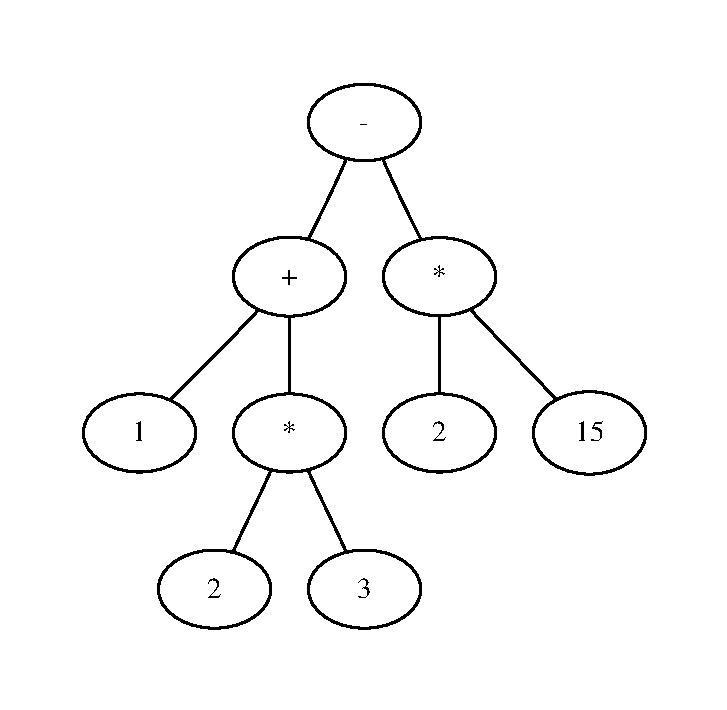
\includegraphics[width=0.5\textwidth]{img/graphs/arithmetic1}
\caption{Arithmetic AST example from the expression \texttt{1+2*3-2*15}}
\label{tree:ast:arithmetic}
\end{figure}

In addition to the operators, rewrite rules have been used in the the more
complex cases where simple operators were not sufficient. This is necessary in
the cases where it is impossible to simply exclude one token, typically in
productions that can produce lists. Figure \ref{code:ast:rewritelist}
illustrates an example for the \verb!letClause! production, where it is only
interesting to preserve the list of variable bindings, which can occur several
times.

\begin{figure}[h]
\begin{verbatim}
letClause : LET varBinding (COMMASi varBinding)*
            -> ^(AST_LETCLAUSE varBinding+);
\end{verbatim}
\caption[AST rewrite rule for the \texttt{letClause} production rule]{Using
rewrite rules to conserve only a list of variable bindings in the AST}
\label{code:ast:rewritelist}
\end{figure}

\subsection{FLWOR expressions}
FLWOR expressions are one of the more complex constructs in XQuery, and
naturally the AST will quickly become complex if care is not taken to include
only the necessary tokens and substrees to preserve information.

On the top level there is the \verb!flWORExpr! production rule, which a
composite of \verb!forClause!, \verb!letClause!, \verb!whereClause!, and
\verb!exprSingle!. Figure \ref{code:ast:flwor} shows the rewrite used for this
production. In this case, a subtree is generated with the imaginary token
\verb!AST_FLOWR! as root. The \$fc and \$lc variables are lists of
for-clauses and/or let-clauses. These are then followed by an optional
where-clause, and an optional orderby-clause. Finally the list of children in
this subtree is terminated by an \verb!exprSingle!, denoting the expression
after the RETURN token.

\begin{figure}[h]
\begin{verbatim}
fLWORExpr : (fc+=forClause | lc+=letClause)+ whereClause?
            orderByClause? RETURN exprSingle
    -> ^(AST_FLWOR $fc* $lc* whereClause? orderByClause? exprSingle);
\end{verbatim}
\caption{AST rewrite rule for FLWOR expressions}
\label{code:ast:flwor}
\end{figure}

In this example we have eliminated a redundant token (\verb!RETURN!) and
condensed the information in the production rule into a subtree more suitable
for traversion, data flow analysis and transformation.

Note however, that this structure is subject to change as requirements may 
emerge. This will be trivial since it is only necessary to edit the rewrite
rule, regenerate the parser, and recompile the program.

The for-clause uses the same technique for augmenting a list of tuplet
definitions, and the child production \verb!forClauseTupletDef! uses simple
operators to exclude superfluous tokens. These rules can be seen in figure
\ref{code:ast:forclause}. 

\begin{figure}[h]
\begin{verbatim} 
forClause : FOR forClauseTupletDef (COMMASi forClauseTupletDef)* 
            -> ^(AST_FORCLAUSE forClauseTupletDef+);

  forClauseTupletDef : DOLLARSi! varName typeDeclaration? positionalVar? 
                     ftScoreVar? IN! exprSingle;
\end{verbatim}
\caption{AST rewrite rule for for-clauses}
\label{code:ast:forclause}
\end{figure}

The let-clause was described earlier in this section, however note that the for-
and let-clauses can be mixed at free will in the FLWOR-expression, so thus
proper care must be taken when parsing the AST. Specifically, special conditions
will apply for determining the number of for- and let-clauses in the expression.
For example, it can be determined that there are no more for/let-clauses when
one encounters one of the following:
\begin{itemize}
  \item \verb!whereClause!
  \item \verb!orderByClause!
  \item \verb!exprSingle!
\end{itemize}

The optional where-clause is trivial. The rewrite rule adds an imaginary
token for clarity and omits the \verb!WHERE! token, as can seen in figure
\ref{code:ast:whereclause}.

\begin{figure}[h]
\begin{verbatim} 
whereClause : WHERE exprSingle
              -> ^(AST_WHERECLAUSE exprSingle);
\end{verbatim}
\caption{AST rewrite rule for where-clauses}
\label{code:ast:whereclause}
\end{figure}

The orderby-clause is also a trivial case. As with the where-clause, an
imaginary token is added for clarity, and the \verb!STABLE! token is preserved
if it is present in the input. In this case, an alternative solution would be to
flag the imaginary root node token as ``stable''. As described in section 
\ref{sect:antlr:ast}, this can be done by subclassing the \verb!CommonTree! (or
\verb!BaseTree!) classes and adding a custom tree adaptor to set such flags on
tokens. The rewrite rule for the orderby-clause is shown in figure
\ref{code:ast:orderbyclause}.

\begin{figure}[h]
\begin{verbatim} 
orderByClause : (ORDER BY | STABLE ORDER BY) orderSpecList
                -> ^(AST_ORDERBYCLAUSE STABLE? orderSpecList);
\end{verbatim}
\caption{AST rewrite rule for orderby-clauses}
\label{code:ast:orderbyclause}
\end{figure}

Finally, the \verb!exprSingle! rule terminates the FLWOR expression. This rule
isa placeholder for any valid expression, and thus it carries no meaning in
itself but rather in the sense of what is deduced from the input.

Figure \ref{tree:ast:flwor1} shows the AST generated for the expression in
figure \ref{code:ast:flwor1}. This is a simple example, but it shows one way to
build an AST for a FLWOR expression.

\begin{figure}[h]
\verbatiminput{graph_queries/flwor1.xq}
\caption{FLWOR expression example, generates AST seen in figure \ref{tree:ast:flwor1}}
\label{code:ast:flwor1}
\end{figure}


\begin{figure}[h]
\centering
 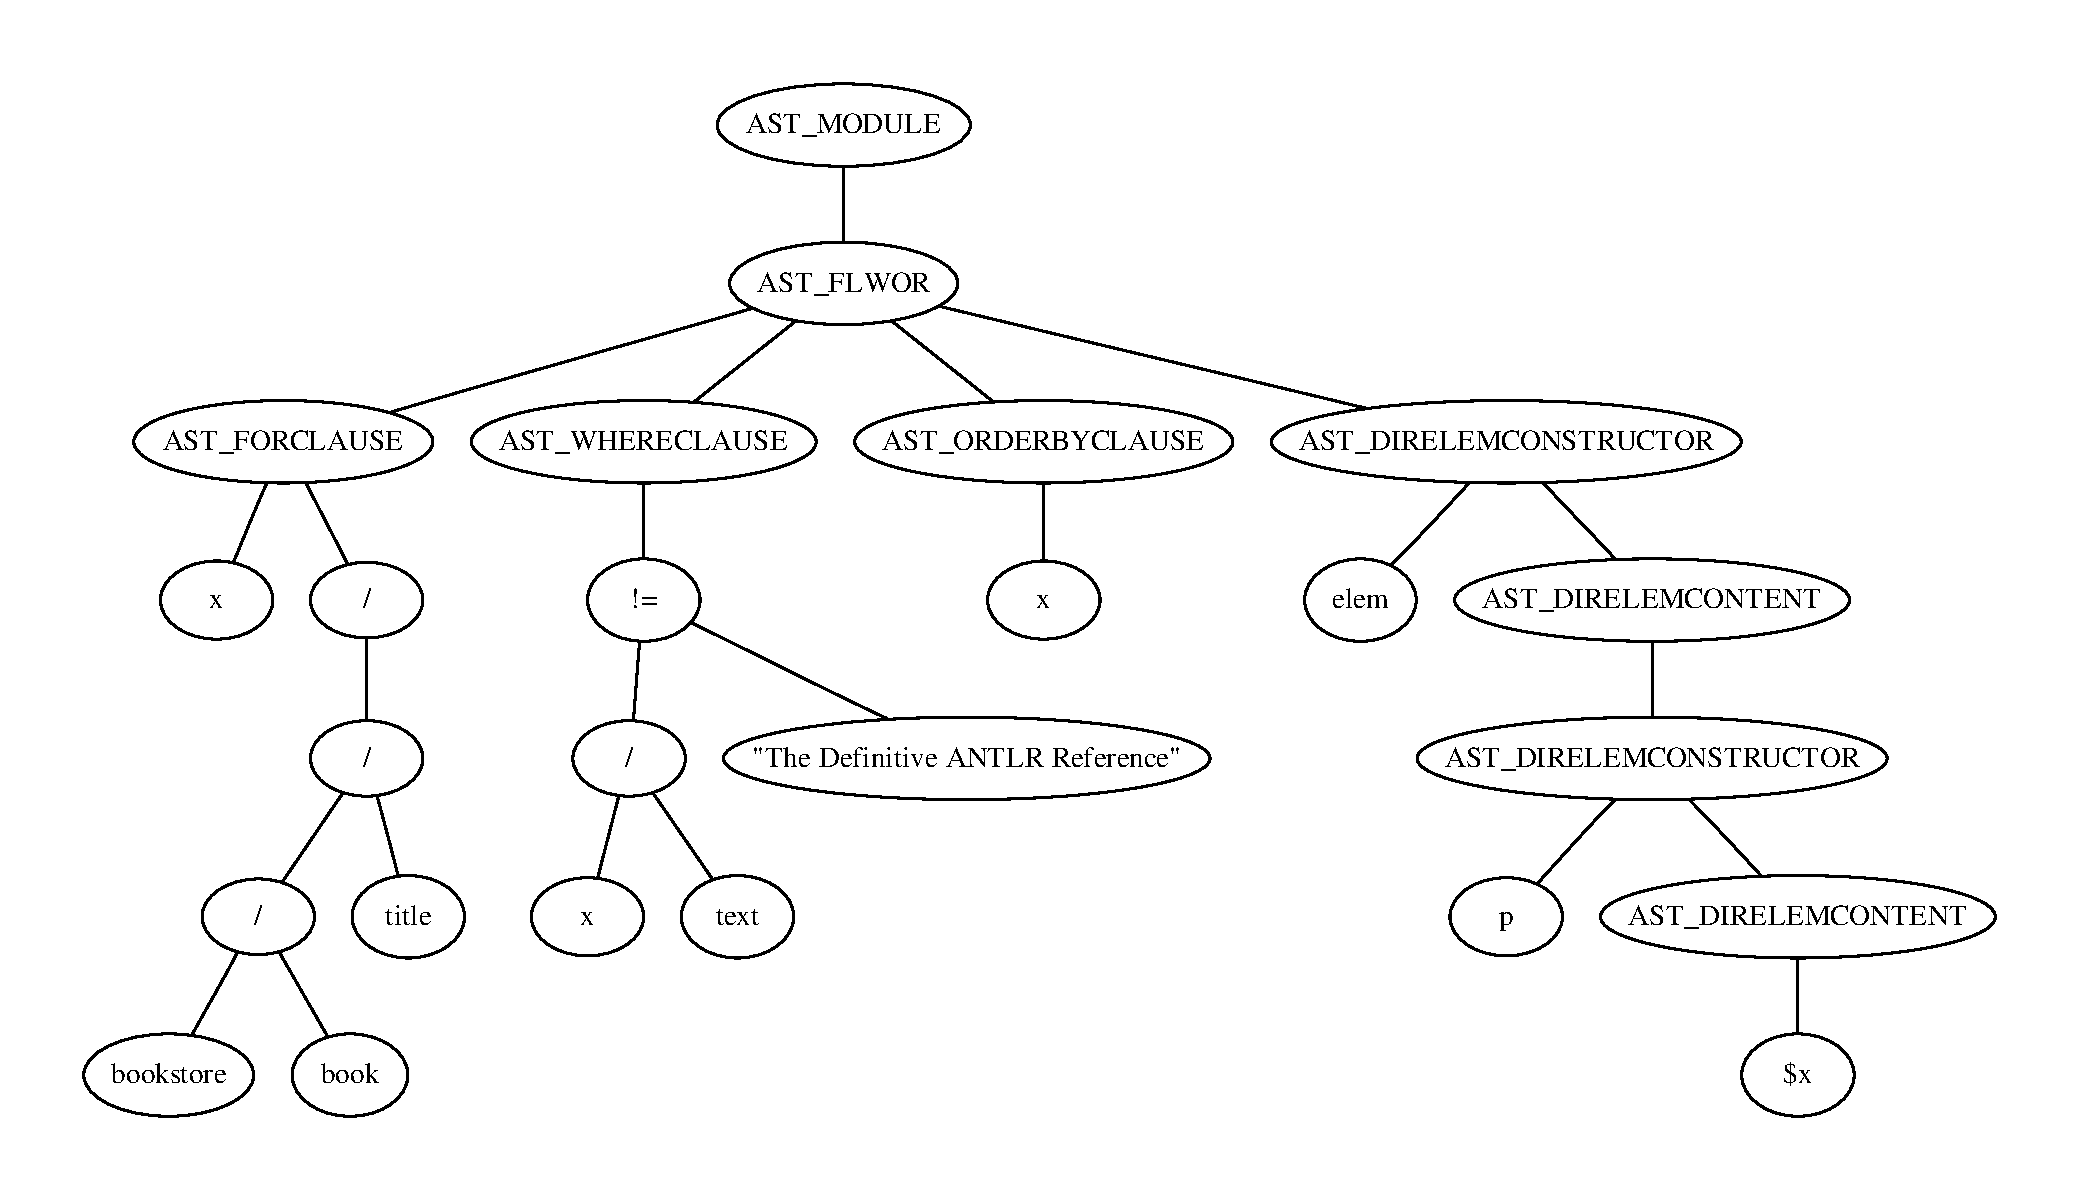
\includegraphics[width=1\textwidth]{img/graphs/flwor1}
\caption{Generated AST tree for FLWOR-expression in figure \ref{code:ast:flwor1}}
\label{tree:ast:flwor1}
\end{figure}


\subsection{Path expressions}
\subsection{Function declarations}
\section{Scoping and symbol tables}
Scoping was implemented using a simple tree structure consisting of parent- and
child scopes. XQuery only allows new scopes to be defined through the
enclosedExpr production rule. This makes it trivial to start a new scope at the
beginning of a enclosedExpr, and end the scope and the end of an enclosedExpr.
This has been implemented as follows:
\begin{figure}[!h]
\begin{verbatim}
enclosedExpr : 
    LBRACESi {
        Scope parent = this.currentScope; 
        this.currentScope = new Scope(); 
        this.currentScope.setParent(parent); 
    }
    expr 
    RBRACSi { 
        this.currentScope = this.currentScope.getParent(); 
    }
;
\end{verbatim}
\caption{Scoping logic embedded in grammar definition}
\end{figure}

Where this.currentScope is a reference to the ``current'' scope in this
context. This member variable is initiated with an empty scope when an object
of the parser class is instantiated.

The implementation above (which is formatted slightly for brevity) will
automatically build a scope tree as the input is parsed.

The currentScope object, which is an object of type Scope, holds one reference
to a symbol table. The symbol table, which is a simple subclass of
java.util.HashMap, is not capable of performing symbol lookups throughout the
scope tree. This functionality is rather provided by the Scope class. This UML diagram
illustrates the relationship between the Scope, SymTab, and Symbol classes:
\clearpage
\begin{figure}[!h]
  \centering
    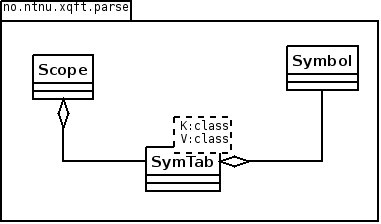
\includegraphics[scale=0.8]{img/uml1}
  \caption{Simplified UML overview of classes related to scope and symbol table}
\end{figure}

\section{Type checking}
XQuery/XPath has a well-defined type hierarchy.
\begin{figure}[h!]
  \centering
    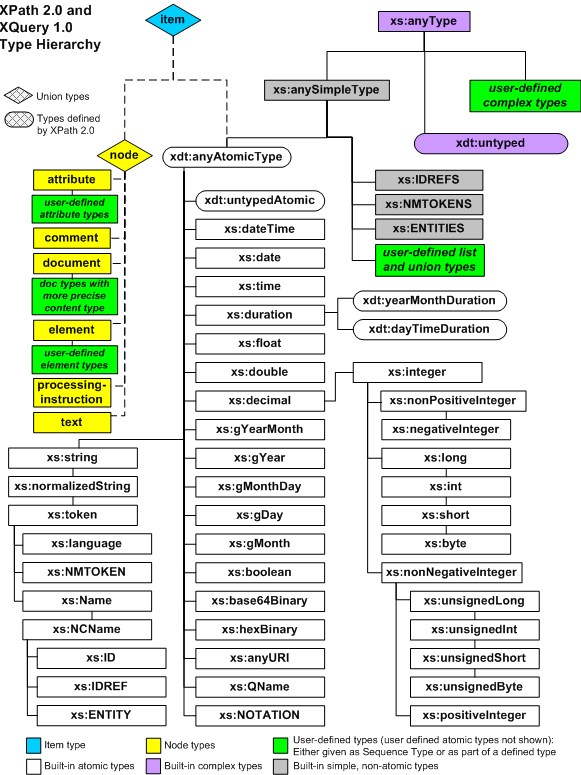
\includegraphics[scale=0.5]{img/xpathtypehierarchy}
  \caption{XQuery/XPath type hierarchy \cite{w3c04} (copyright
  \copyright W3C)}
\end{figure}
Here is a short overview of the basic type system:
\begin{itemize}
  \item Node types
    \begin{itemize}
      \item element()
      \item attribute()
      \item text()
      \item commment()
      \item document-node()
      \item processing-instruction()
    \end{itemize}
  \item Structure types
    \begin{itemize}
      \item Atomic types (xs:integer, xs:string, ..)
      \item Simple types (list, union)
      \item Complex types (user-defined types from an XML schema, except
      xs:anyType and xdt:untyped)
    \end{itemize}
\end{itemize}

Atomic types are strongly typed except xs:untypedAtomic, xs:anyURI, as well as
numerical types (xs:integer, xs:double, ..). Non-atomic simple types as well as
complex types are both strongly typed.

Proper type checking requires implementation of type inference and type
synthesis. This requires a stable abstract syntax tree and advanced data flow
analysis techniques to be feasible. Due to the inherent limitations in this
project, type checking has not been implemented - however the possibility of
this is discussed in section \ref{sect:summary:future_work}.

\underline{\textbf{\LARGE //TODO:}}
\begin{itemize}
  \item Dynamic vs. Static typing
  \item Strong vs. Weak (what and when)
  \item Type inference
  \item Michael Rys
\end{itemize}

\underline{\textbf{\LARGE //ODOT:}}
% ERROR HANDLING
\section{Error Handling}
\subsection{Syntax errors}
\label{sect:error_handling:syntax_errors}
As mentioned in section \ref{sec:impl:errorhandling}, error handling was added
by forcing ANTLR into throwing exceptions upwards to the calling program.

However, it quickly became appareant that some of the errors in the lexer were
not discovered by the parser, and no exceptions were thrown for these errors. The
lexer would simply print an error message to stderr, consume the offending
character, and attempt recovery. This led to complications when running the
XQuery Test Suite (see section \ref{sect:tests:manual}).


% Implementation / Coverage tests
% Andreas, hei andreas!
\section{Manual Compliance Tests}
\label{sect:implementation:manualCoverage}
The XQuery test suite supplied by W3C\cite{w3c05} consists of a number of
XQuery query files, and a corresponding set of output files with expected
output/result for queries where this applies. Additionally, a central XML file
describing all the tests with references to files and folders are also supplied.

This file was parsed using a simple implementation of the reference SAX API
from the SAX project website\cite{saxproject}. For each applicable
test case, a new parser was instantiated and executed on the input file. If the
parser succeeded without throwing an exception, the test was considered passed.
This measurement of ``success'' was proposed in section \ref{sect:method:testing}.

Note that by ``applicable'' it is implied only tests which could be executed in
parse-time. That is, some tests require run-time features such as type
checking. This premise was presented in section \ref{sect:method:testing}.

The level of compliance was calculated by counting the number of passed tests, and
simply computing the percentage.


\section{Summary}
In this chapter we have gone through by which means we chose to adapt the W3C
XQuery Full-text specification to ANTLR syntax and semantics. We chose to adapt
the specification over creating our own from scratch because the otherwise risk
of missing out essential latent meaning as well as timely concerns, as
discussed further in section \ref{sect:discussion:adaptW3C}.    

By choosing to implement an "parser controlled state driven" lexer (section
\ref{sect:amiguousgrammar:parserControlled}), almost all terminal productions
had to be completly rewritten, and also lead to the introduction of the
\verb!TOKENSWITCH! construct. This could be avoided by implementing e.g. a
"scan-while-parse" type lexer, but such a lexer's corresponding parser would
have been much more complex and would handle a much bigger load than that of
our implementation. A more viable alternative would be the "island grammars"
strategy, but because ANTLR does not support this we rejected this solution. In
section \ref{sect:discussion:designDecisions} we further evaluate our choice of
lexer strategy.         

We also implemented enclosed composite lexer productions which removed a great
deal of terminal ambiguities by moving the whole refering non-terminal rule
into the lexer. The container tokens were introduced to lessen the strain on
the parser.   

W3C specifies some extra-gramatical contraints for XQuery Full-text. Our parser
comply with a great deal of these, however, there are still some
unconformities, as discussed in section \ref{sect:future:knownBugs}.  

We have described the implementation of AST rewrite rules and operators to have
ANTLR generate a complete AST shaped after these rules and operators. We also
examined several XQuery constructs such as FLWOR and path expressions and how
the AST were to be generated for these.

Further we have detailed the implementation of symbol tables and scoping. We
discovered that it was simple to add inline code in the grammar to extend the
parser with these features, however it may seem like this is affecting
readability and clarity of the grammar. In the next chapters this issue will be
further examined and discussed.

As we now have seen how the parser was implemented, in the next chapter we will
se how it performs, in particular with regards to coverage test results, AST
output, and error handling.
